%
% File: chap01.tex
% Author: Victor F. Brena-Medina
% Description: Introduction chapter where the biology goes.
%
\let\textcircled=\pgftextcircled
\chapter{Introduction}
\label{chap:intro}

\initial{S}haring economy, \textit{the peer-to-peer-based activity of obtaining, giving, or sharing the access  to  goods  and  services,  coordinated  through community-based online services} \cite{hamari2015sharing}, is a very important phenomenon grown exponentially over the last decade. Building trust in these online marketplaces is the key to the adoption of sharing economy. Even though all the markets require some minimum amount of trust, for Internet markets this is a particular challenge considering the fact that trades are typically anonymous, geographically dispread and executed sequentially \cite{owen2014trust}. To incentivize trustworthiness, online markets employ feedback mechanisms, which allow traders to share opinions about past experiences. Online feedback mechanisms, also known as reputation systems, \textit{have emerged as a viable mechanism for fostering cooperation among strangers in such settings} \cite{dellarocas2003digitization}. Examples of these systems, for instance eBay, Amazon or AirBnb, after each trade, encourage both parties to give feedback about their trading partner based on their experience. 

For online marketplaces to succeed and prevent a market of lemons, their feedback technologies must be able to not only collect users feedback, but to properly analyze it and differentiate among sellers. The most common types of feedback are ratings and text comments.  An important separation between the distinct role of text comments as tacit knowledge and explicit feedback ratings. According to \cite{pavlou2006nature}, text comments are particularly interesting for the audience as a new trust-building means in online marketplaces, which reveals hidden knowledge that cannot be described by negative/positive ratings. 

A survey by \cite{pavlou2006institutional} asked the respondents to indicate how many feedback comments they examined for the seller they purchased from.before each transaction they did online. The result showed that 81\% reported examining 25 comments (one webpage), 5\% viewed 50 comments, 11\% more than 50 ones, and only 3\% did not examine any text comments. This finding reveals that despite the importance of text feedback to the users, it is apparently difficult for the them to access the meaning of numerous text comments for a single item \cite{pavlou2006institutional}.
Let us consider an example of a person who is searching for accommodation in the Airbnb site. The user really wants the room to be quiet, no more than 5 min walking from the public transport station and to have good Wifi connection. In order to find information about all these features the user has to check several options and to read the comments of each of them, in order to identify the required features. Given this situation, the average human reader will have difficulties on identifying and extracting the relevant information from the opinions in them Automated sentiment analysis systems are thus needed \cite{liu2012sentiment}.



\section{Customer Focus Theory}
\label{sec:CFTH}

When offering a service or product, it is essential to understand what consumers' preferences are and how can we shape the offerings accordingly to create value. Customer Focus Theory is one of Information Studies theories, which specifically offers a guide on how to put the focus on the customer. This theory should be explained according to the context of my research (where it is placed and adds value on the framework) as shown in Figure \ref{fig:CustomerFocus}. 
--- Narrow down to "Receiving and utilization of customer feedback" and the accordance with the research topic.

% This is a requirement of Business Information Studies track: Base and support the thesis research on one (or more) of Information Studies theories. Link: http://is.theorizeit.org/wiki/Main_Page 
\begin{figure}[t!]
	\centering
	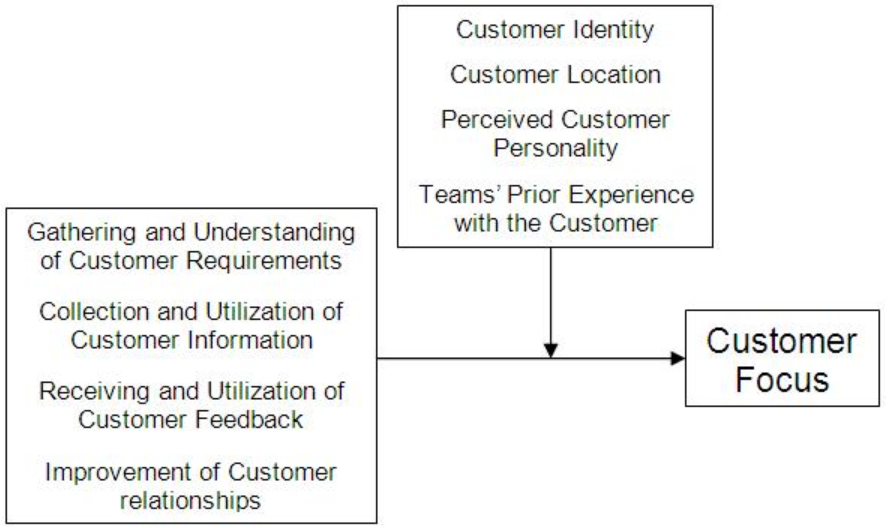
\includegraphics[height=0.3\textheight]{fig01/CustomerFocus}
	\caption{Theoretical framework of Customer Focus theory}
	\label{fig:CustomerFocus}
\end{figure}

\section{Online Feedback systems}
\label{sec:OFS}

\subsection{Principles of OFS and game theory}

Various mechanisms have been designed and utilized
in C2C auction markets to promote trust and reduce risk.
For instance,
eBay's “Feedback Forum” is a form of community enforcement.
In eBay, after each trade, both buyers and
sellers are encouraged to leave comments about their
trading partners based on their experience. Comments
about traders are kept under each trader's profile, and can
be accessed by everyone who visits eBay. This way, the
system tries to deter dishonest behavior by conveying
facts and opinions about past trades. Kollock [15]
conceptually summarizes online reputation systems and
concludes that their effectiveness to manage the risks of
unsecured trades seems to be impressive. Resnick et al.
[20] review the online reputation systems and argue that
the reputation systems appear to perform reasonably well
despite their theoretical and practical difficulties. \cite{yang2007effects}


\subsection{Characteristics of most popular OFSs}
\label{subsec:popularOFS}

This subsection will explain how online feedback systems work. In addition, it will describe, categorize and point out the differences between the typical types of OFS used by the most successful online marketers (Ebay, Amazon, Yelp, TripAdvisor and Airbnb). 

\subsection{Methods for analyzing customer feedback}
\label{subsec:feedbackmethods}
This subsection will mention the methods how the customer feeback can be analyzed in order to get the most out of it. The ratings and the text reviews will be explicitely mentioned in order to create the right environment for jumping to the problem statement.

\subsection{Bias in the OFSs}
\label{subsec:bias}
Explains the phenomenon of bias in the online feedback systems and also the different types of bias noticed in them. The subsection will end up to the bias that this research aims to reduce.

\textit{Preliminary:} Many academic papers on online reputation systems and building trust in the online marketplace report the existence of bias on online reviews [1, 3, 4, 5, 6, 9], therefore reducing the bias of these systems is an important issue towards a more efficient online feedback system. 

\section{Problem statement}
\label{sec:problemstatement}
This section will clearly define the problem and the research question at the end.The first subsection focuses on the methods proposed to move toward a more efficient feedback system.

\subsection{Three ways to move toward a more efficient OFS}
\textit{Preliminary:} In 2008 the giant of online marketplaces eBay changed radically the way how their feedback system was working. Many researchers have analyzed the eBay changes \cite{fradkin2016bias,resnick2006value,bolton2013engineering,dini2009buying,dellarocas2008sound}, and findings suggest three ways to move toward a more efficient feedback system. A solution would be to mitigate to a new validated feedback system and follow it strictly. However abandoning the existing system and move to a new one requires a lot of effort and sometimes the model also does not fit considering the differences in the type of transactions. The second solution suggested is to build channels of feedback in a targeted way, for example only one side feedback or the element of anonymousness. The third solution learnt from the eBay case suggests using complementary methods for feedback analysis. This third solution offers in itself a lot of potential considering the big variety of tools for data analysis. This paper proposes text mining of reviews as a complementary method for feedback analysis in the reputation systems. 

\subsection{Feature based opinion mining}
This subsection will introduce the concept of sentiment mining and how it can be used for analysing the text of customer feedback in online feedback systems.

\subsection{Research question}
\textit{Preliminary:} Text reviews as part of the feedback in the online marketplace have a big importance for the users of
these platforms, which is often underestimated from their owners. Research in the field suggest that text
opinions influence the users’ decisions even when the rating for the listing is high \cite{fradkin2016bias}. Furthermore, the
study of the Airbnb feedback systems argues that a negative rating is followed by a text in 45\% of the cases,
which implies the great power of text mining for discovering the negative features of the listing. The methods for doing so fall into the category of sentiment based opinion mining methods. Examples of their application include mainly the movie rating systems (Netflix, IMDb) and the product rating systems (eBay).
This research proposes the implementation of sentiment based opinion mining methods as complementary for the review analysis in the online feedback systems of the accommodation market, explicitly in the Airbnb feedback system.
This research is based mostly on the question: “How can sentiment-based opinion mining methods complement the analysis of reviews in an online reputation system?” The research aims to test the methods which can effectively calculate the reputation scores of the text reviews and afterwards find the ways how these methods can be integrated with the current methods of feedback analysis. To be more precise, the Airbnb system calculates now the overall rating for a listing based on the average score of at least three reviews and this score has a proven bias (tend to be always positive). Given the fact that text reviews reveal often the negative aspects of the listing, generating a low score of feedback for them and calculating this score in the overall rating, will we reduce the bias? I believe that the answer is yes, however in order to have an answer for these questions the research is planned as described in the next section.